
\documentclass[10pt, %
showfigures % uncomment for final submission (figures get uploaded separately)  
]{jneurosci}
% small bibliography
\usepackage{jneurosci}

\newcommand{\loremipsum}{Lorem ipsum dolor sit amet, consectetur adipisicing elit, sed do eiusmod tempor incididunt ut labore et dolore magna aliqua. Ut enim ad minim veniam, quis nostrud exercitation ullamco laboris nisi ut aliquip ex ea commodo consequat. Duis aute irure dolor in reprehenderit in voluptate velit esse cillum dolore eu fugiat nulla pariatur. Excepteur sint occaecat cupidatat non proident, sunt in culpa qui officia deserunt mollit anim id est laborum.}

%% --------- DOCUMENT --------------------------------------------------

\title{Your fancy title}
\date{\normalsize\today}
\author{Me And\textsuperscript{1}, You Blub}

\begin{document}
\maketitle
\begin{affiliations}
\item Your University
\end{affiliations}

\begin{frontpage}

  \item[Running title:] 
  \item[Corresponding Author:] ~\\
Me And, PhD\\
Your university and adress\\
\item[Number of pages:]
\item[Number of figures:]
\item[Number of tables:]
\item[Number of words Abstract:]
\item[Number of words Introduction:]
\item[Number of words Discussion:]
\item[Conflict of Interest:] The authors declare no competing financial interests.
\item[Acknowledgements:] 
\end{frontpage}

\begin{abstract}
\loremipsum
\end{abstract}


\begin{introduction}
\loremipsum
\begin{figure}
  \begin{center}
    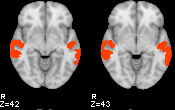
\includegraphics[width=.5\textwidth]{examplefig}
  \end{center}
  \caption{This is an example figure. Show or hide with option \texttt{showfigures}.}
\end{figure}

\nocite{*}
\end{introduction}

\begin{methods}
\loremipsum
\end{methods}

\begin{results}
\loremipsum
\end{results}


\begin{discussion}
\loremipsum
\end{discussion}

% The \references command creates section heading if needed, and
% clears the page if needed
\references{ex_jneurosci}

\listoffigures
\end{document}
